% -*- root: ../main.tex -*-
%!TEX root = ../main.tex
% this file is called up by main.tex
% content in this file will be fed into the main document
% vim:textwidth=80 fo=cqt

\subsection{The transfer operator and its model form}
In a classical system identification  task, the discrete-time transfer functions
for the systems  under consideration need to be  determined. These discrete-time
transfer functions are  based on Z-transforms in the  frequency domain. However,
for the purpose of working in time-domain, an analogous linear operator $q$ that
performs a  forward shift on  its input \ie{} $  {q u[k] \longmapsto  u[k+1]} $.
Similarly, applying the  backward shift operator $ q^{-1} $  on the input yields
its value at the previous time-step \ie{} $ {q^{-1} u[k] \longmapsto u[k-1]}$.

\begin{figure}[!htb]
    \centering
    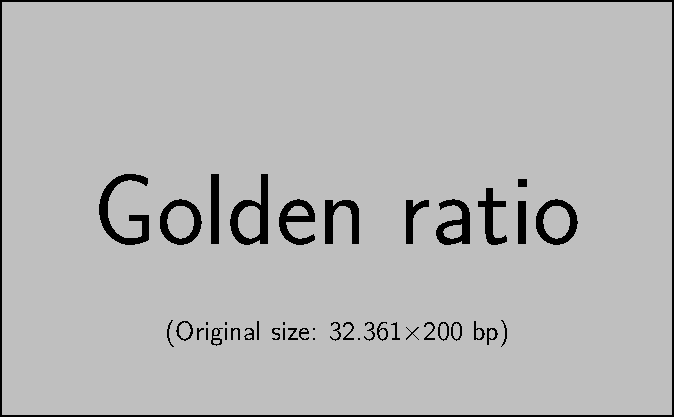
\includegraphics{placeholder_images/example-image-golden.pdf}
    \caption[Block diagram representing a generic discrete-time \glsfmtshort{lti} system]{%
        Block  diagram representing  a  generic discrete-time  \glsfmtshort{lti}
        system. The  control input $u[k]$ is  acted upon by the  system dynamics
        $G[k]$  whereas a  white  noise  input $e[k]$  is  shaped  by the  noise
        dynamics $H[k]$. The  overall output $y[k]$ consists  of a superposition
        of the contribution from both these components.
    }%
    \label{fig:genericltisyswithnoise}
\end{figure}

\Cref{fig:genericltisyswithnoise} shows  a generic \gls{lti} system  wherein the
measurements are corrupted by noise. The  system dynamics are represented by the
transfer operator $G(q)$\footnote{The term transfer  operator in the time domain
mathematically  corresponds  to the  term  transfer  function in  the  frequency
domain.  Mathematically,  $G(q) =  G(z)\bigr\rvert_{\mathrlap{z=q}}$.}  that  acts on  the
applied  input  $u[k]$,  whereas  the  noise dynamics  are  represented  by  the
disturbance operator  $H(q)$ that  acts to  filter (or  shape) an  assumed white
noise input $e[k]$.

Assuming linearity and time-invariance throughout, the overall output can be
written as the linear combination
\begin{equation}\label{eq:outputwithsysandnoise}
    % \SwapAboveDisplaySkip
    y[k] = G(q)u[k] + H(q)e[k]
\end{equation}
where $G(q) = \frac{B(q)}{A(q)}$ and $H(q) = \frac{C(q)}{D(q)}$ are the transfer
operators describing the dynamics of the system and disturbance respectively.

$A(q), B(q), C(q)$ and $D(q)$ are rational polynomials in $q$. The two transfer
operators $G(q)$ and $H(q)$ can be represented by
\begin{align}
    G(q) &= q^{-n_k}\frac{b_1q^{-1} + \dots  + b_{n_b}q^{-{n_b}}}{1 + a_1q^{-1} + \dots  + a_{n_a}q^{-{n_a}}} \\
    H(q) &= q^{-n_l}\frac{c_1q^{-1} + \dots  + c_{n_c}q^{-{n_c}}}{1 + d_1q^{-1} + \dots  + d_{n_d}q^{-{n_d}}}
\end{align}
where $(n_k,n_l)$ represent  the number of transport  delay samples, $(n_b,n_c)$
the number  of feedforward coefficients  and $(n_a,n_d)$ the number  of feedback
coefficients in $G(q)$ and $H(q)$ respectively.


In  this  system  identification  task  at hand,  the  output  measurements  are
collected from a  \emph{noise-free} simulation of the \gls{p2d}  model \ie{} the
disturbance transfer operator in~\cref{eq:outputwithsysandnoise} is zero
\begin{align}
    y[k] &= G(q)u[k] + \cancelto{0}{H(q)}e[k]
\shortintertext{Hence, the time-domain output  reduces  to}
    y[k] &= G(q)u[k]
\end{align}

Thus, the system identification task becomes one that of estimating
\begin{enumerate}
    \item The number of transport delay samples $n_k$.
    \item The number of feedforward coefficients (zeros) $n_b$.
    \item The zeros themselves $b_1, b_2, \dots b_{n_b}$.
    \item The number of feedback coefficients (poles) $n_a$.
    \item The pole locations $a_1, a_2 \dots a_{n_a}$.
\end{enumerate}
for  each  of  the  two  transfer operators  $G_1(q)$  and  $G_2(q)$  \ie{}  the
electrolyte  time-evolution subsystems  in the  negative and  positive electrode
region respectively.

\subsection{Estimation of transport delay}

The transport delay $n_k$ can be estimated visually by inspecting the step
response of the systems under consideration.

In~\cref{fig:linearity},   step  inputs   of   $I_1   =  \SI{60}{\ampere},   I_2
=    \SI{12}{\ampere},$   and    $I_3   =    \SI{36}{\ampere}$   were    applied
to    the   two    subsystems.    Inspecting   closely    all   the    responses
\ie{}   $\widetilde{Q}_{\text{e,n}_1},    \widetilde{Q}_{\text{e,n}_2}   $   and
$\widetilde{Q}_{\text{e,n}_3}$    in    the     negative    electrode    region,
and    $\widetilde{Q}_{\text{e,p}_1},    \widetilde{Q}_{\text{e,p}_2}   $    and
$\widetilde{Q}_{\text{e,p}_3}$  in the  positive electrode  region, it  is clear
that all these outputs start exactly at  zero. Therefore, there is no delay term
to be considered for the transfer operators \ie{} $n_k = 0$ for both subsystems.

\subsection{Choice of model structure}

Among      the      transfer-function       model      structures      mentioned
in~\cref{subsec:parametric}, the \gls{arx} model  structure is too simplistic to
consider. Despite  the fact that  its numerical computation involves  only basic
linear algebra operations,  that can be efficiently handled  on modern computing
systems, it  is considered to produce  poor estimates of the  system's poles and
zeros. In the absence of contributions from the noise-term, the all-encompassing
model structure used by the Box-Jenkins approach is deemed to be unnecessary for
the  problem  at hand.  Therefore,  the  two  model structures  considered  were
\gls{armax} and \gls{oe} for the coefficient determination.

\begin{figure}[!htb]
    \centering
    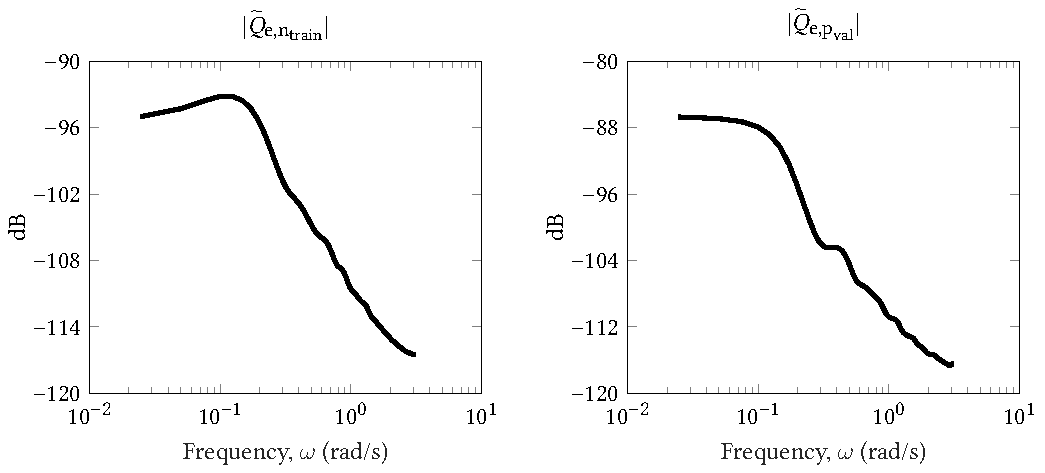
\includegraphics[width=\textwidth]{bode_mag.pdf}
    \caption{}
    \label{fig:initialbodemag}
\end{figure}
